\documentclass[a4paper]{article}

\usepackage[english]{babel}
\usepackage[utf8]{inputenc}
\usepackage{amsmath}
\usepackage{graphicx}
\usepackage[colorinlistoftodos]{todonotes}
\usepackage{caption}
\usepackage{subcaption}
\usepackage{here}

\title{Computational Photography}

\author{Mich\`ele Wyss, 10-104-123}

\date{December 11, 2014}

\graphicspath{{imgs/}}
\begin{document}
\maketitle

\section*{Ray space analysis}
\section*{EPI's}
Some example EPI's can be seen in Figure \ref{fig:EPIs}. 
The slopes of the lines vary with the depth of the object. 
For example, in the EPI of scanline 40, it's very well visible that the pink lines have a very different slope than all the other lines. 
This is because the pink animal is much closer to the camera than the rest and therefore seems to move faster when the camera drives by.
\begin{figure}[ht]
	\begin{subfigure}[h]{0.48\textwidth}
	  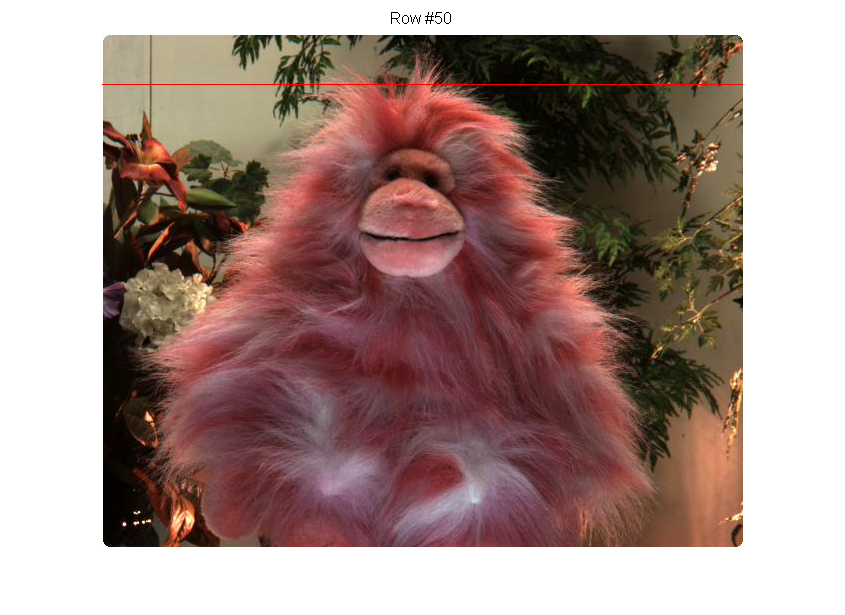
\includegraphics[width=\textwidth]{scanline50}
	  \caption*{Scanline at row 50}
	\end{subfigure}
    	~
	\begin{subfigure}[h]{0.48\textwidth}
	  \centering
	  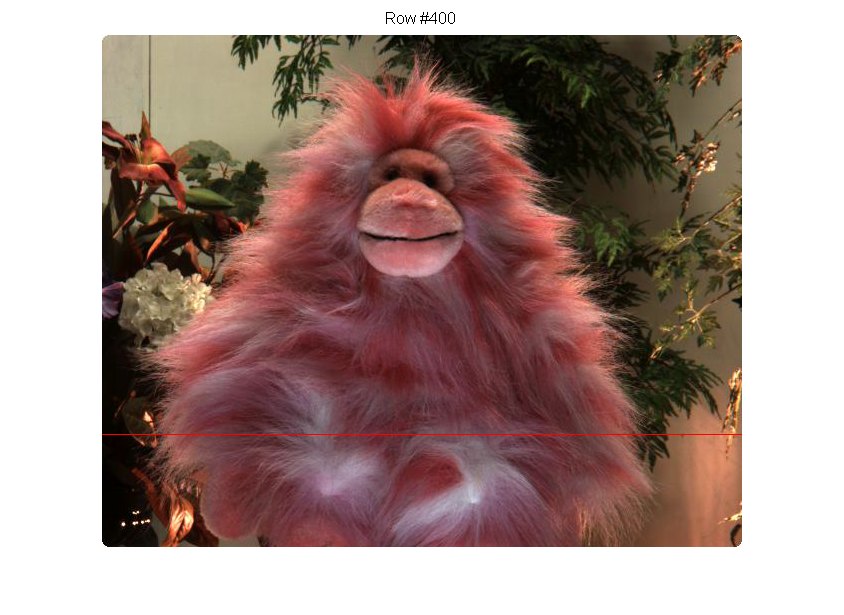
\includegraphics[width=\textwidth]{scanline400}
	  \caption*{Scanline at row 400}
	\end{subfigure}
	
	\vspace{2mm}
	\begin{subfigure}[h]{0.48\textwidth}
	  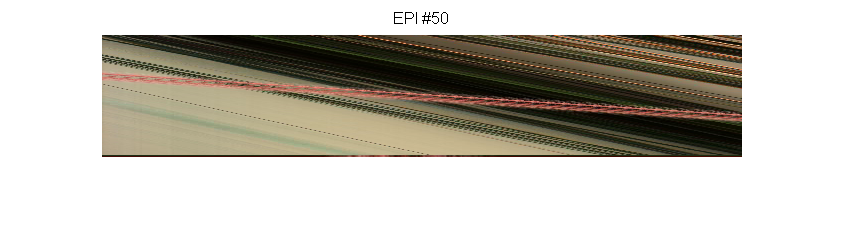
\includegraphics[width=\textwidth]{EPI50}
	  \caption*{EPI at 50}
	\end{subfigure}
    	~
	\begin{subfigure}[h]{0.48\textwidth}
	  \centering
	  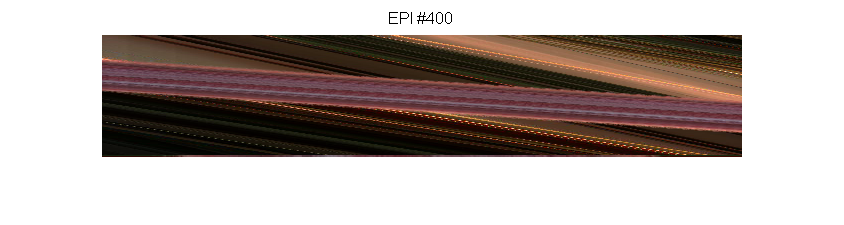
\includegraphics[width=\textwidth]{EPI400}
	  \caption*{EPI at row 400}
	\end{subfigure}
\caption{Examples of EPI's at two different scanlines of the pink animal scene.}
\label{fig:EPIs}
\end{figure}
\section*{Fourier Transform and visualized power spectrum}
\todo{What can be observed on the images? How can the images be interpreted?}
For the same scanlines as above, the Power spectrum of the two EPI's is visualized in Figure \ref{fig:powerSpectrum}
\begin{figure}[ht]
	\vspace{2mm}
	\begin{subfigure}[h]{0.48\textwidth}
	  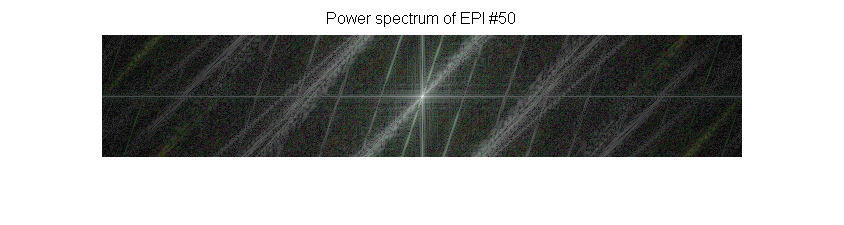
\includegraphics[width=\textwidth]{powerSpec50}
	  \caption*{Power spectrum at 50}
	\end{subfigure}
    	~
	\begin{subfigure}[h]{0.48\textwidth}
	  \centering
	  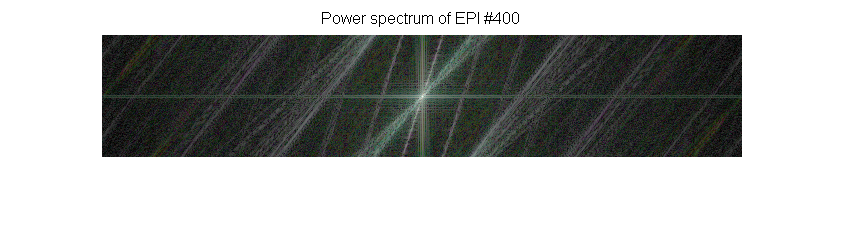
\includegraphics[width=\textwidth]{powerSpec400}
	  \caption*{Power spectrum at 400}
	\end{subfigure}
\caption{Visualized power spectrum of the two EPI's at scanlines 50 and 400.}
\label{fig:powerSpectrum}
\end{figure}
\end{document}